% This is "sig-alternate.tex" V1.9 April 2009
% This file should be compiled with V2.4 of "sig-alternate.cls" April 2009
%
% This example file demonstrates the use of the 'sig-alternate.cls'
% V2.4 LaTeX2e document class file. It is for those submitting
% articles to ACM Conference Proceedings WHO DO NOT WISH TO
% STRICTLY ADHERE TO THE SIGS (PUBS-BOARD-ENDORSED) STYLE.
% The 'sig-alternate.cls' file will produce a similar-looking,
% albeit, 'tighter' paper resulting in, invariably, fewer pages.
%
% ----------------------------------------------------------------------------------------------------------------
% This .tex file (and associated .cls V2.4) produces:
%       1) The Permission Statement
%       2) The Conference (location) Info information
%       3) The Copyright Line with ACM data
%       4) NO page numbers
%
% as against the acm_proc_article-sp.cls file which
% DOES NOT produce 1) thru' 3) above.
%
% Using 'sig-alternate.cls' you have control, however, from within
% the source .tex file, over both the CopyrightYear
% (defaulted to 200X) and the ACM Copyright Data
% (defaulted to X-XXXXX-XX-X/XX/XX).
% e.g.
% \CopyrightYear{2007} will cause 2007 to appear in the copyright line.
% \crdata{0-12345-67-8/90/12} will cause 0-12345-67-8/90/12 to appear in the copyright line.
%
% ---------------------------------------------------------------------------------------------------------------
% This .tex source is an example which *does* use
% the .bib file (from which the .bbl file % is produced).
% REMEMBER HOWEVER: After having produced the .bbl file,
% and prior to final submission, you *NEED* to 'insert'
% your .bbl file into your source .tex file so as to provide
% ONE 'self-contained' source file.
%
% ================= IF YOU HAVE QUESTIONS =======================
% Questions regarding the SIGS styles, SIGS policies and
% procedures, Conferences etc. should be sent to
% Adrienne Griscti (griscti@acm.org)
%
% Technical questions _only_ to
% Gerald Murray (murray@hq.acm.org)
% ===============================================================
%
% For tracking purposes - this is V1.9 - April 2009

\documentclass{sig-alternate}

\usepackage{url}
\usepackage{soul}

%for scribbles to myself
\usepackage{color}

%for the DRAFT watermark
%\usepackage{graphicx}
%\usepackage{type1cm}
%\usepackage{eso-pic}
%\usepackage{color}
%\makeatletter
%\AddToShipoutPicture{%
%            \setlength{\@tempdimb}{1\paperwidth}%
%            \setlength{\@tempdimc}{1\paperheight}%
%            \setlength{\unitlength}{1pt}%
%            \put(\strip@pt\@tempdimb,\strip@pt\@tempdimc){%
%        \makebox(600,-800){\rotatebox{45}{\textcolor[gray]{0.75}%
%        {\fontsize{6cm}{6cm}\selectfont{DRAFT}}}}%
%            }%
%}
%\makeatother

\begin{document}
%
% --- Author Metadata here ---
%\conferenceinfo{WOODSTOCK}{'97 El Paso, Texas USA}
%\CopyrightYear{2007} % Allows default copyright year (20XX) to be over-ridden - IF NEED BE.
%\crdata{0-12345-67-8/90/01}  % Allows default copyright data (0-89791-88-6/97/05) to be over-ridden - IF NEED BE.
% --- End of Author Metadata ---

%\title{Middleware for Aiding the Creation of Cross Reality Environments}

%\title{A Taxonomy of System Support for Cross Reality}

%\title{The State of Cross Reality}

%\title{The State of Cross Reality and its Applicability to Exploration of Cultural Heritage}

%\title{Cross Reality for Cultural Heritage}

\title{Virtual Time Windows: Applying Cross Reality to Cultural Heritage}

%\title{Real and virtual world copresence with cross reality intercommunication for exploration of cultural heritage sites}

%\title{Alternate {\ttlit ACM} SIG Proceedings Paper in LaTeX Format}
%\titlenote{(Produces the permission block, and
%copyright information). For use with
%SIG-ALTERNATE.CLS. Supported by ACM.}}
%\subtitle{[Extended Abstract]
%\titlenote{A full version of this paper is available as
%\textit{Author's Guide to Preparing ACM SIG Proceedings Using
%\LaTeX$2_\epsilon$\ and BibTeX} at
%\texttt{www.acm.org/eaddress.htm}}}
%
% You need the command \numberofauthors to handle the 'placement
% and alignment' of the authors beneath the title.
%
% For aesthetic reasons, we recommend 'three authors at a time'
% i.e. three 'name/affiliation blocks' be placed beneath the title.
%
% NOTE: You are NOT restricted in how many 'rows' of
% "name/affiliations" may appear. We just ask that you restrict
% the number of 'columns' to three.
%
% Because of the available 'opening page real-estate'
% we ask you to refrain from putting more than six authors
% (two rows with three columns) beneath the article title.
% More than six makes the first-page appear very cluttered indeed.
%
% Use the \alignauthor commands to handle the names
% and affiliations for an 'aesthetic maximum' of six authors.
% Add names, affiliations, addresses for
% the seventh etc. author(s) as the argument for the
% \additionalauthors command.
% These 'additional authors' will be output/set for you
% without further effort on your part as the last section in
% the body of your article BEFORE References or any Appendices.

\numberofauthors{2} %  in this sample file, there are a *total*
% of EIGHT authors. SIX appear on the 'first-page' (for formatting
% reasons) and the remaining two appear in the \additionalauthors section.
%
\author{
% You can go ahead and credit any number of authors here,
% e.g. one 'row of three' or two rows (consisting of one row of three
% and a second row of one, two or three).
%
% The command \alignauthor (no curly braces needed) should
% precede each author name, affiliation/snail-mail address and
% e-mail address. Additionally, tag each line of
% affiliation/address with \affaddr, and tag the
% e-mail address with \email.
%
% 1st. author
\alignauthor
CJ Davies\\%\titlenote{}\\
       \affaddr{University of St Andrews}\\
%       \affaddr{1932 Wallamaloo Lane}\\
%       \affaddr{Wallamaloo, New Zealand}\\
       \email{cjd44@st-andrews.ac.uk}
% 2nd. author
%\alignauthor
%Alan Miller\\%\titlenote{The secretary disavows any knowledge of this author's actions.}\\
%       \affaddr{University of St Andrews}\\
%       \affaddr{P.O. Box 1212}\\
%       \affaddr{Dublin, Ohio 43017-6221}\\
%       \email{alan@cs.st-andrews.ac.uk}
}
% There's nothing stopping you putting the seventh, eighth, etc.
% author on the opening page (as the 'third row') but we ask,
% for aesthetic reasons that you place these 'additional authors'
% in the \additional authors block, viz.
%\additionalauthors{Additional authors: John Smith (The Th{\o}rv{\"a}ld Group,
%email: {\texttt{jsmith@affiliation.org}}) and Julius P.~Kumquat
%(The Kumquat Consortium, email: {\texttt{jpkumquat@consortium.net}}).}
\date{19 September 2011}
% Just remember to make sure that the TOTAL number of authors
% is the number that will appear on the first page PLUS the
% number that will appear in the \additionalauthors section.

\maketitle
\begin{abstract}
This paper provides an overview of the `cross reality' paradigm $-$ the fusion of ubiquitous sensor/actuator infrastructure and virtual environments facilitating synchronous bidirectional intercommunication between real and virtual worlds, allowing each to reflect, influence and merge with the other. We recount the history of the concept, explain its situation in relation to other alternate realities that computer science has explored, survey existing commercial and research implementations, and propose its suitability to furthering the application of alternate realities to the domain of cultural heritage.

We present the Virtual Time Window concept, a new endeavour applying cross reality to cultural heritage intending to make use of the recently released ISO/IEC 23005 (MPEG-V) framework to address the issue of standards in achieving synchronous bidirectional intercommunication between the heterogeneous constituent technologies of ubiquitous sensor/actuator infrastructure and virtual environments.
\end{abstract}

% A category with the (minimum) three required fields
\category{C.2.4}{Computer-Communication Networks}{Distributed Systems}
%A category including the fourth, optional field follows...
%\category{D.2.8}{Software Engineering}{Metrics}[complexity measures, performance measures]

\terms{Measurement, Standardization.}

\keywords{Cross reality, mixed reality, augmented reality, augmented virtuality, sensor, actuator, virtual environment, virtual world, ISO/IEC 23005, MPEG-V, cultural heritage.}

\section{Introduction}
\label{sec:introduction}
One application of 3D virtual environments, including virtual worlds such as Second Life and game/visualization engines such as Unity3D, is the simulation of real world locations~\cite{wright:duality}. By introducing readings from sensors distributed throughout a real world location into a virtual environment that hosts a simulation of that location, the simulation's state can be made to respond in real time to physical and environmental changes in the real world; temperature, humidity, movement, etc. Inversely, changes to the state of the simulation, perhaps caused by an user-controlled avatar or by automated scripts, can be made to affect the real world by use of actuators; controlling HVAC systems, door openers, Representation of Sensory Effects (RoSE) devices~\cite{Timmerer2009}, etc.

This synchronous combination into a single system of augmented virtuality (affecting a virtual environment according to information from the real world)~\cite{Want2009} and augmented reality (affecting the real world according to information from a virtual environment)~\cite{Want2009} gives rise to a specific mixed reality situation referred to more precisely as \textit{cross reality}~\cite{Coleman2009}.

There are currently no widely adopted standards, frameworks nor approaches for this synchronous intercommunication of sensory and control information between real and virtual environments in pursuit of cross reality. Previous endeavours~\cite{Lifton2007a, mit:doppel, Coleman2009, UgoTrade2007, wright:duality, Yankelovich2009, IBM2008, Marketwire2008} have relied upon bespoke designs and implementations, requiring substantial additional work in bringing together the disparate constituent technologies before novel uses and applications of the paradigm can be explored.

ISO/IEC 23005 (MPEG-V)~\cite{InternationalOrganizationforStandardization2011}, published in its 1st edition on April 1$^{st}$ 2011, aims to alleviate this issue, however it is still too early to ascertain how well it will achieve this and whether it will succeed in garnering widespread support.

This paper proceeds in section \ref{sec:crossreality} by defining cross reality and describing its position in relation to other alternate realities explored by computer scientists, then investigates the applicability of alternate realities and particularly the cross reality paradigm to the domain of cultural heritage in sections \ref{sec:alternaterealityincultheritage} and \ref{sec:crossrealityincultheritage}, including details of previous research conducted at St Andrews into the use of virtual worlds in cultural heritage scenarios. The Virtual Time Window project is introduced in section \ref{sec:vtwintro}.

\section{Cross Reality}
\label{sec:crossreality}
Cross reality is the ubiquitous mixed reality environment that rises from the fusion of sensor/actuator (collectively `transducer'~\cite{Song2008}) infrastructure and virtual environments, where augmented reality and augmented virtuality manifest simultaneously to facilitate synchronous multi-directional exchange of media and control information between real and virtual environments. Sensors collect and tunnel dense real-world data into virtual environments where they are interpreted and displayed to dispersed users, whilst interaction of virtual participants simultaneously incarnates into the real world through a plenitude of diverse displays and actuators~\cite{Paradiso2009, Coleman2009}. Cross reality is also referred to by some authors as X-reality~\cite{kim:practical}.

The paradigm was founded in work conducted by Joshua Lifton whilst part of the Responsive Environments Group at MIT's Media Lab, initially adopting the name `dual reality' ~\cite{Lifton2009, lifton:adoption};

\begin{quotation}
	\textit{``An environment resulting from the interplay between the real world and the virtual world, as mediated by networks of transducers. While both worlds are complete unto themselves, they are also enriched by their ability to mutually reflect, influence and merge into one another''}~\cite{Lifton2007a, lifton:merging}.
\end{quotation}

Whilst these inaugural projects and much of the successive work in the field has made use of virtual worlds such as Second Life, OpenSimulator (OpenSim) and Open Wonderland, there are no features inherent to virtual worlds and unavailable to more traditional 3D game and visualization packages that make the latter unsuitable for realizing the paradigm. However the combination into a single piece of software of a multi-user 3D environment, rudimentary 3D modelling capabilities and a simple scripting language makes virtual worlds a more accessible alternative to cross reality researchers than traditional 3D game and visualization solutions, as the latter often require experience in a complex standalone 3D modelling package in order to create content for even a rudimentary environment.

\subsection{Background to Alternate Realities}
Due to the nature of cross reality it is useful to review some of the rich set of alternate realities that computer science has invented and explored.

\begin{itemize}
	\item \textbf{Virtual reality} $-$ An environment that is entirely virtual and completely immersing, allowing the user to interact with a completely synthetic world~\cite{Milgram1999}; a new world that exists solely within the data structures of a computer~\cite{Want2009}.
	\item \textbf{Augmented reality} $-$ A real environment onto which digital information is overlain ~\cite{Want2009}. A commercial example is the Layar browser~\cite{eishita:layar} for mobile phones, which overlays various forms of data onto the view captured by a phone's camera after determining its location and orientation using GPS, accelerometer and digital compass.
	\item \textbf{Augmented virtuality} $-$ A synthetic environment onto which information from the real world is overlain~\cite{caballero:behand}. A simple example is the EyeToy accessory and associated software for Sony's Playstation 2 games console $-$ a digital camera that captures images of players and their surroundings and integrates them into the gaming experience presented on the screen.
	\item \textbf{Mixed reality} $-$ An environment created by the merging of real and virtual environments to some extent, such that the result is neither entirely real nor entirely synthetic, where real and virtual objects co-exist~\cite{Want2009}.
\end{itemize}

Describing all environments that are neither entirely real nor entirely virtual, mixed reality is a relatively generic term that encompasses both augmented reality and augmented virtuality. This concept is illustrated by Milgram's \textit{virtuality continuum}, included as figure \ref{virtualitycontinuum}, which comprises a linear scale situating an entirely real, completely non-modelled environment at one extremum (the real world) and an entirely virtual, completely modelled environment at the opposite extremum (virtual reality), with mixed reality constituting everything inbetween~\cite{Milgram1994}.

\begin{figure}[h!tbp]
\centering
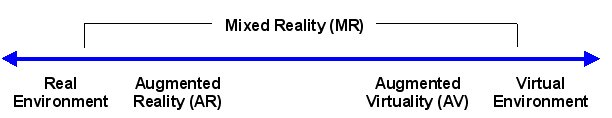
\includegraphics[width=0.48\textwidth]{virtualitycontinuum.jpg}
\caption{Milgram and Kishino's \textit{virtuality continuum}.}
\label{virtualitycontinuum}
\end{figure}

`Modelled' refers to the computer's knowledge of the environment it is presenting; with an entirely real environment the computer associates no knowledge or meaning to any of the objects presented, whilst in an entirely virtual environment the computer associates meaning with every object that it is presenting. Between these extremes the computer associates meaning with some objects, but not all; in the case of augmented reality for example, meaning is associated with the digital objects it is overlaying atop the real environment, but not with the real environment itself.

These different categories of alternate realities can also be visualised in two dimensions as shown in figure \ref{virtualitymatrix} (based on a similar figure that appeared in~\cite{Want2009}).

\begin{figure}[h!tbp]
\centering
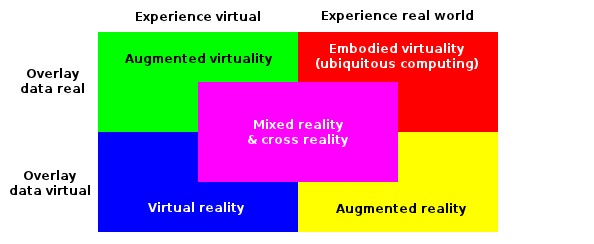
\includegraphics[width=0.56\textwidth]{virtualitymatrix.png}
\caption{A 2x2 matrix that visualises the relationship between different classifications of alternate realities.}
\label{virtualitymatrix}
\end{figure}

\subsection{The Position of Cross Reality}
A cross reality system comprises two environments, one augmented reality and the other augmented virtuality. Presumably the reason for its original title of dual reality, this is also why it cannot be positioned at any single point along the virtuality continuum; the two constituent environments occupy different positions. It is the combination of these two environments into a single system, such that there is media and control information being exchanged between them simultaneously and in both directions, that creates cross reality;

\begin{quotation}
	\textit{``The important point of X-reality is a conceptual paradigm shift from single-directional information flows to bidirectional information flows between two worlds.''}~\cite{kim:practical}
\end{quotation}

It is worth noting that this definition does not stipulate that the information or media being shared between the two environments be of the same type or magnitude.

{\section{Examples of Cross Reality Systems}
There have been numerous successful cross reality projects to date, both research and commercial. The following represents a brief survey of some of the most influential.

\subsection{MIT Responsive Environments Group~\cite{MIT}}
Mentioned in section \ref{sec:crossreality}, the Responsive Environments Group at MIT's Media Lab was responsible for some of the inaugural work in defining the field of cross reality and continues to actively research the paradigm to this day.
	
	Their Dual Reality Lab project~\cite{Lifton2007a, lifton:merging} that started in 2006 investigated virtual and real worlds that reflect, influence and merge into each other by means of a deeply embedded bespoke transducer network comprising power strips imbued with sensing, computational and communicative capabilities~\cite{Lifton2007b}.
	
	The Dual Reality Lab evolved into the cross reality initiative and the 2008 Ubiquitous Sensor Portal project, in which a network of 45 such `Portals' distributed throughout the Lab, each equipped with an array of sensors in addition to a touch screen display, loudspeaker and camera, permitted 2-way audio and video communication between people in the real Lab and avatars in its virtual counterpart in Second Life~\cite{Lifton2009}.
	
	DoppelLab~\cite{mit:doppel}, the Group's latest cross reality project, is investigating the use of the game engine Unity3D to browse and interact with data from densely-deployed transducer networks.	
	
\subsection{Eolus One~\cite{Coleman2009, UgoTrade2007}}
A project from Swiss construction, building services and real estate company Implenia, involving creative minds from  IBM, SAP, Wago and Zumtobel, that ran for 2 years exploring concepts including Building Automation Systems (BAS), energy monitoring, alert management and preventive maintenance. Eolus One connected real-time data collection and distributed control mechanisms of smart buildings in the real world to a Virtual Command Center (VCC) hosted in Second Life. This connection was facilitated by a bespoke hardware and software platform, the Virtual World Communication Interface (VWCI), which mediated communication between Second Life and various protocols in BAS, including ZigBee, CANOpen and Modbus.

	This resulted in a 20 to 27 percent reduction in energy consumption and carbon footprints of buildings under this control, attributed to improvements in the manner in which data streams from multiple systems (heating, cooling, water usage, fuel consumption) could be combined, visualized, analysed, tracked and interacted with, even leading to discovery of previously unknown issues that were not apparent from studying streams individually. These improvements also reduced the manpower requirements for monitoring large numbers of buildings, as an individual operator was able to assimilate more information.
	
\subsection{IBM 3-D Data Center~\cite{IBM2008, Marketwire2008}}
In 2008 IBM announced their 3-D Data Center technology allowing the recreation of data centres in secure virtual worlds, bringing real-time data from different facilities into a 3D environment to visualize hot spots, data flow, server utilization and more to reduce cost, save time and help reduce carbon footprints.
	
	Implenia made use of these solutions to extend the functionality of their existing VCC by using IBM's virtual world integration middleware, Holographic Enterprise Interface (HEI), to add data from datacentre equipment to their existing virtual world models. Before the advent of this IBM technology Implenia's knowledge of the state of their data centres comprised only of information from BAS and their VWCI, with no information from the servers themselves.
	
	By introducing this information to their existing models, Implenia were allowed a finer control of HVAC and security systems, allowing them to take action to be more efficient, with the consolidated views giving their operators insight into real physical issues such as how heat and energy flow through the data centre.

\subsection{6thSpace~\cite{Yankelovich2009}}
A 2009 project from Malden Labs that used Sun's Project Wonderland virtual world (now the Open Wonderland project) to allow remote system administrators to collaborate with on-site staff to diagnose problems with computer equipment, with the remote participants gaining access to terminal windows on the on-site hardware by leveraging Wonderland's application-sharing feature.
	
	This same application-sharing feature has been investigated by groups of scientists, remotely controlling laboratory equipment and visualising results in 3D by interfacing with external data sources, enabling collaborative lab-based research to be undertaken by geographically dispersed researchers~\cite{Fayolle2011}.

\section{Alternate Realities in Cultural Heritage}
\label{sec:alternaterealityincultheritage}
The use of alternate realities in the domain of cultural heritage has been an area of active research for over 20 years as it provides many advantages over more traditional techniques employed for the capture, analysis and in particular the presentation and visualization of the domain material~\cite{Roussou2002}.

A number of such projects are identified by~\cite{walczak:applications}. The majority of this research has focussed on the application of augmented reality and virtual reality to aiding in the presentation, visualization and thus accessibility of information to both experts and interested novices, such as visitors to museums and sites of interest. These applications have been employed to;

\begin{itemize}
	\item visualize and provide (remote) access to sites and artefacts that no longer exist, never existed or only exist in a damaged or decayed state, are hard or impossible to reach (both due to physical and legislative reasons, the latter often due to items being held in private collections) or are the result of speculation (time, distance, scale, etc.)~\cite{griffin:recovering, deamicis:gamebased, Christou2006, Laycock2008, Dikaiakou2003, willmott:largecomplex, roussou:photorealism, Levoy1999, levoy:digitalmichelangelolong};
	
	\item quickly and easily present and explore multiple representations of sites and artefacts, allowing domain experts to compare, contrast and test different theories of reconstruction, restoration and relocation and also to aid in the analysis process that generates new understanding by allowing the available information to be studied in fashions that are not possible using traditional approaches, such as easily visualizing changes through time~\cite{Ikeuchi2003, cabral:x3dexperience, griffin:recovering, Laycock2008, Sundstedt2004, mcnamara:lightness, Levoy1999, levoy:digitalmichelangelolong};
	
	\item aid accessibility and increase interest, particularly in children who can be easily underwhelmed and lose interest when presented with sites that no longer represent their former glory, and aid distance learning and education~\cite{deamicis:gamebased, ardito:combining, Seo2010, Kim2009, roussou:photorealism};

	\item enable informal methods of education and research; interactive, collaborative and responsive, and enable different modalities of interaction with the information, such as haptics~\cite{deamicis:gamebased, Christou2006, benko:collaborative};

	\item digitally preserve sites and artefacts that are in danger of decay~\cite{Ikeuchi2003, Remondino2009, Levoy1999, levoy:digitalmichelangelolong};

	\item reduce complexity of creating presentations and visualizations, so that once information that pertains to a site or artefact has been collected the process of preparing it for presentation to users is a less involved and expert affair~\cite{Ruffaldi2008, roussou:photorealism};

	\item improve the standard of audiovisual tours of sites, such that they better reflect the users' current position, gaze, etc. without restricting them to a predetermined path, only providing information at pre-chosen points of interest, or requiring excessive prompting to, or control from, the user~\cite{Seo2010, Kim2009, vlahakis:archeoguide}.
\end{itemize}

The success of these projects, establishing a strong research base for alternate reality in cultural heritage, paves the way for investigation into applications of the cross reality paradigm to the domain.

\subsection{Virtual Worlds and Cultural Heritage at St Andrews}
Research has already been conducted at St Andrews into the use of virtual worlds for projects within the domain of cultural heritage. These include reconstructions in OpenSim of a Byzantine basilica in the Sparta region of Greece~\cite{Getchell2010} (see figure \ref{basilicascreenshot}) and of the cathedral at St Andrews~\cite{UniversityofStAndrewsComputerScienceblog2011} (see figure \ref{cathedralscreenshot}).

Both of these sites now lie in ruins so virtual reconstructions, that allow people to explore them as they were at their prime, allow for rewarding modalities of interaction and can lead to the deduction of new knowledge that was not apparent from other techniques of study.

For example, the basilica reconstruction has allowed experts to explore the interior of the building to investigate how lines-of-sight at different points in the building played such an important role in its design, something that was not previously possible from studying maps, plans and static viewpoint reconstructions.

In March this year we are presenting the reconstruction of the cathedral both to school students and to members of the general public, making use of projection screens and investigating the use of video game controllers to control avatars in a more familiar fashion for many, particular younger, users than the somewhat `clunky' keyboard and mouse controls of Second Life viewers.

\begin{figure}[]
\centering
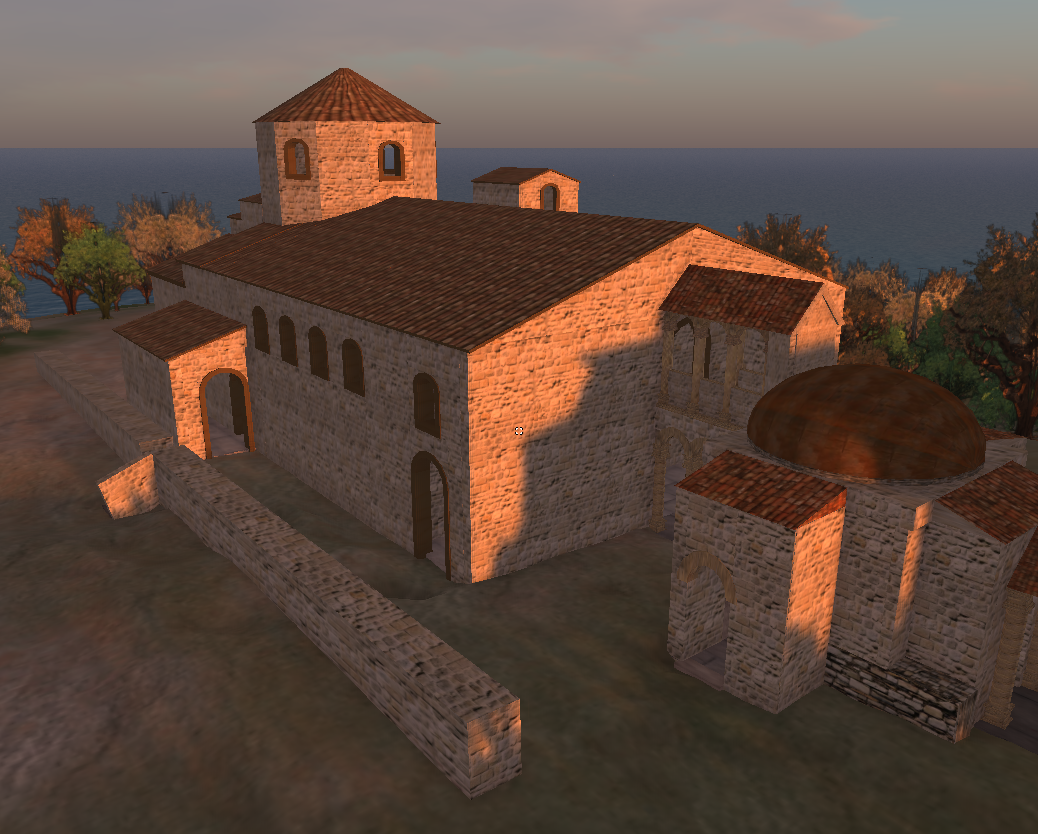
\includegraphics[width=0.48\textwidth]{basilicascreenshot.png}
\caption{OpenSim reconstruction of a Byzantine basilica in the Sparta region of Greece.}
\label{basilicascreenshot}
\end{figure}

\begin{figure}[]
\centering
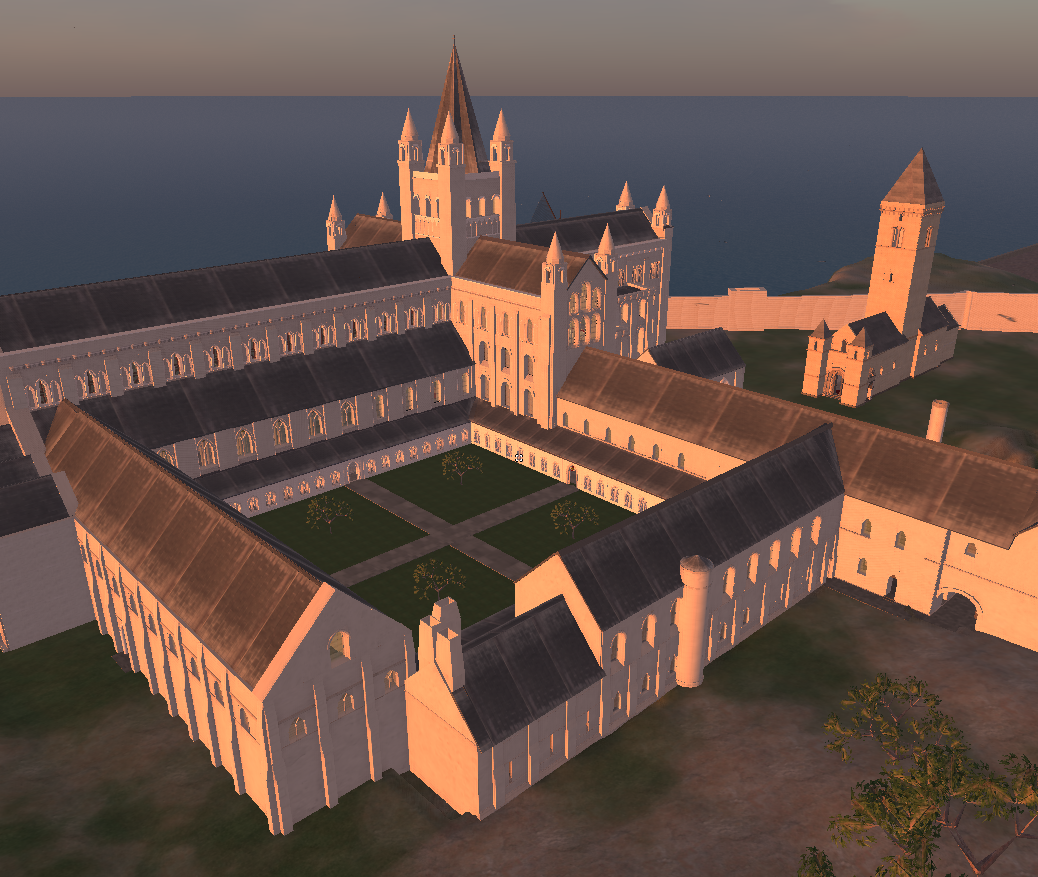
\includegraphics[width=0.48\textwidth]{cathedralscreenshot.png}
\caption{Reconstruction of the cathedral at St Andrews, as it was during the 1300's.}
\label{cathedralscreenshot}
\end{figure}

\section{Cross Reality in Cultural Heritage}
\label{sec:crossrealityincultheritage}
Cross reality promises to expand upon existing alternate reality research in the domain of cultural heritage by increasing the level of interactivity between users, artefacts and sites, by coupling real world conditions more tightly to those pertaining to the digital content of the site and vice-versa, allowing each to influence the other to a greater degree.

The following is a brief overview of several areas in which cultural heritage is particularly well suited to benefit from cross reality, though it should not be considered an exhaustive survey.

\subsection{User Interaction with Digital Content}
\label{subsec:userinteraction}
Many of the projects referenced in section \ref{sec:alternaterealityincultheritage} use augmented reality to overlay digital content atop the user's view of a real world site. Interaction with this content is often very limited, where included at all, and there are few common modalities between different sites that feature such systems.

A cross reality approach in which the digital content is hosted within the context of a wider 3D virtual environment, allowing the user the full freedom of control offered by a virtual world avatar or game player character, permits a much greater level of interactivity and involvement between users and augmentations. Artefacts can be `picked up' for closer examination and passed between different users to aid more natural discussion and collaborative learning, as well as dynamically changing their representation in real-time in response to commands from users, such as changing from an assembled view to an exploded view to aid in the understanding of complex mechanisms and construction. Users can take copies of artefacts, storing them in the inventory system of the virtual environment for further study at a later time, even once they have left the site (see section \ref{subsec:remoteaccess}).

\subsection{Real World Influencing Digital Content}
Augmented reality implementations usually present users with digital content comprising static models rendered with prebaked textures. Combined with a lack of sensing capabilities this results in content that cannot dynamically change in relation to changing physical and environmental conditions at the site, such as lighting and weather. As a result there is a marked continuity error between the digital content and the surrounding real environment whenever the conditions in the latter do not match those adopted during the creation of the former.

For example, if a ruined building is digitally modelled in its original splendour as if in sunlight and then rendered atop a user's view of the ruins in the real world, the model will merge well with the surrounding real environment only if the user visits the site during fair weather. If the user visits the site during torrential rain the quality of their experience will be lessened due to the rendered reconstruction not merging as well with its surroundings.

Cross reality allows for readings from environmental sensors dispersed about the site to affect the digital content presented to users, such that the appearance of the content better reflects the current site conditions. This dynamic alteration ranges from simple control of lighting direction onto surfaces of digital content to reflect the passage of the Sun across the sky throughout the day, to more complex representations of weather conditions such as rain, snow and mist.

\subsection{Digital Content Influencing Real World}
As previously identified, alternate reality deployments in the domain of cultural heritage have focussed on the use of augmented reality and virtual reality to present visual and auditory content to users. There has been comparatively little research into the presentation of complete somatosensory content, including physical changes to the state of a site through control of lights, fans, heaters, RoSE devices, etc. Cross reality allows for actions and events that take place within the virtual environment to trigger such changes in the state of the site, allowing content to address more sensory systems and opening a vast range of new modalities of interaction between users and digital content.

A simple example is of a user altering the lighting conditions of a digital component within the virtual environment (see section \ref{subsec:userinteraction}) and these same alterations manifesting in the real site through the use of a remotely controllable lighting fixture via the DMX512 protocol~\cite{Technology} or similar. This particular example could make it much easier for a user to map between features of a real artefact and the coinciding features of its digital reconstruction.

\subsection{Extent of Digital Content}
\label{subsec:extentdigital}
The majority of previous augmented reality deployments in cultural heritage have added sparse digital objects to users' views of a site, resulting in easily identifiable augmentations that `stand out' from their real surroundings due to their imperfect photorealism. By hosting these digital objects within a larger virtual environment they will no longer appear out of place, as the level of photorealism of the objects themselves will be identical to that of the virtual environment around them, presenting a more consistent experience.

Creating an entire virtual environment, instead of only certain objects of interest to add to the site, also gives rise to different possible modalities of interaction between visitors and digital content. Because a surrounding virtual environment gives context to the objects, they can be observed and interacted with solely in the virtual environment or alongside the site, instead of having to be `mixed' with the site in the traditional sense of augmented reality. Of course there is nothing to prevent these same objects from also being used in this traditional fashion, by allowing them to be accessed independently of their virtual surroundings.

\subsection{Remote Access to Digital Content}
\label{subsec:remoteaccess}
The digital content of most cultural heritage sites that employ alternate reality technologies is only accessible to users who are physically present at the site. In the case of virtual reality deployments this content is usually delivered using a bespoke or proprietary platform that is not commonly or freely available to individuals, whilst for augmented reality content it is a defining feature of the concept that this content be overlayed upon a direct or indirect view of the real site, something that is not usually available remotely. Whilst some sites may present a subset of their digital content to remote users via a website, possibly employing techniques such as panoramic photographs, this is a markedly different and more limiting style of interaction than that of alternate realities.

By employing cross reality and modelling not only particular objects of interest but also the environment surrounding them (see section \ref{subsec:extentdigital}), the digital content becomes useful in a standalone situation as well as becoming remotely accessible. This ability to remotely access, using freely available software such as a virtual world client on a standard home computer, the same virtual environment as is used to present visitors to the site itself with digital content, either alongside their view of the real site using a tablet or handheld computer, or mixed with their view of the site using an augmented reality glasses approach, raises interesting possibilities with regards to interaction between users at the site and remote users.

Visitors to the site can be guided by a domain expert who is not physically with them at the site, but who is logged in to the virtual environment at a computer elsewhere. Similarly visitors to the site can invite friends and family who are unable to accompany them to the site to `join' them, by logging into the virtual environment, as they explore and learn about the site.

Remote access to the virtual environment also promises to extend users' interaction with the site beyond the end of their physical visits, whilst retaining familiarity with the methods of presentation. Upon returning home, users can share their experiences at the site with their friends and family by logging in to the virtual environment from their home computer, perhaps instead of showing them photographs they had taken at the site. If a user discovered after leaving the site that they missed something, or ran out of time to see everything that they wanted to, or simply wished to revisit a certain artefact, they can log in to the virtual environment at a later point to see it.

\section{Virtual Time Window Project}
\label{sec:vtwintro}
We are working on a novel application of the cross reality paradigm to the exploration of cultural heritage sites in a project dubbed the Virtual Time Window (VTW), which aims to investigate the use of tablet computers to present visitors to a cultural heritage site with a `window' into a virtual world based reconstruction of the entire site as it was at an earlier point in time. This allows visitors to alternate at will between viewing the site in its current state around them and in its earlier state through the window, facilitating simultaneous exploration of real and virtual worlds. Figure \ref{vtwmockup} illustrates this concept.

The project is currently in its initial phases, as we survey and acquire necessary hardware and software, familiarise ourselves with their development environments and begin to write some of the back end support utilities.

\begin{figure}[]
\centering
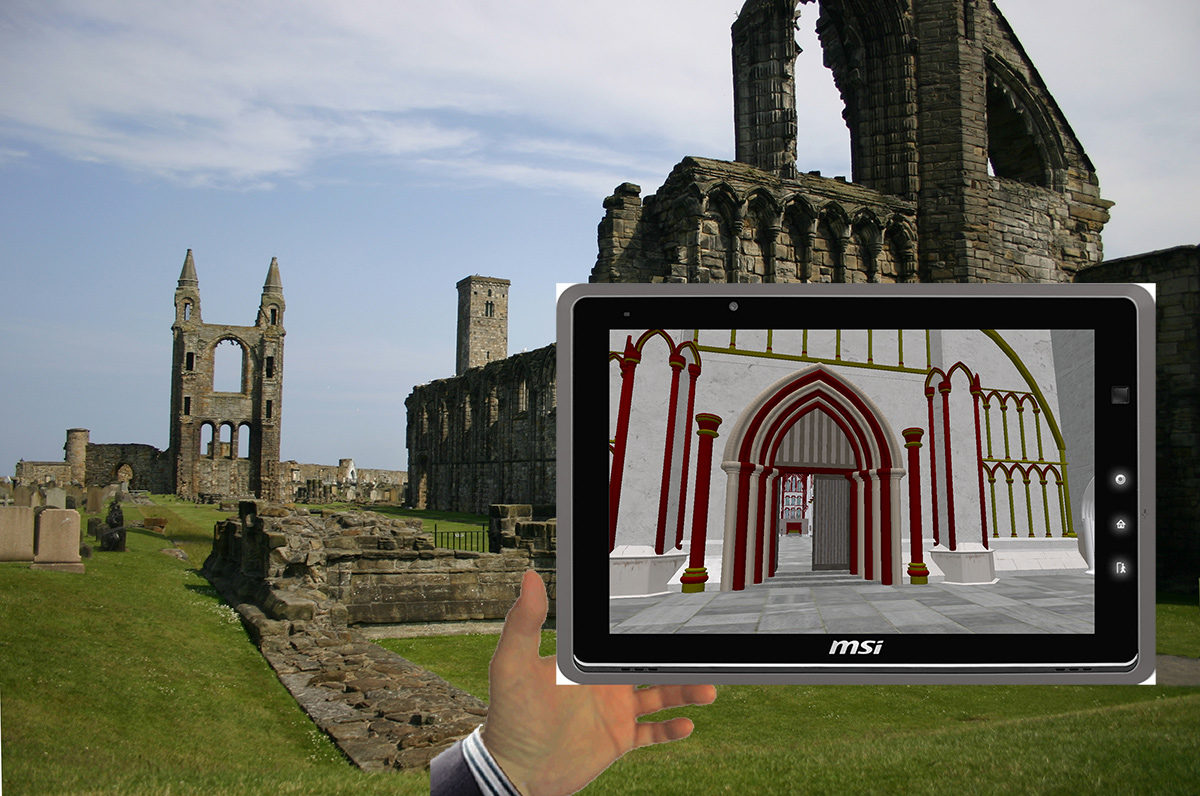
\includegraphics[width=0.48\textwidth]{mockup.jpg}
\caption{Illustration of VTW concept.}
\label{vtwmockup}
\end{figure}

\subsection{Overview of VTW}
\label{subsec:overviewofvtw}
The VTW concept maintains a natural manner of exploration as it does not require visitors to manually control movement of avatar or camera in the virtual world, nor does it restrict exploration to predefined paths or areas.

A visitors' movement around the site is reflected by equivalent movements of an avatar around the virtual world. This mimicry will make use of GPS, possibly using DGPS beacons/reference stations, in combination with digital compass. If it is discovered that the accuracy attainable from this combination is insufficient, additional location tracking technologies will be employed; image recognition/visual tracking frameworks are an obvious candidate and their use within the context of cultural heritage sites has already received investigation~\cite{Seo2010}.

Change in orientation of a tablet is reflected by corresponding change to the orientation and focus of the camera belonging to a particular avatar, making use of accelerometer and digital compass. When a visitor wishes to see what a particular object or area looked like in the past, or wishes to access other digital information that may pertain to their current location and a particular gaze, they simply raise the window and look through it in a manner akin to composing a photograph using the screen on the back of a digital camera.

Furthermore, environmental and other physical properties of the site are captured by sensor infrastructure and these data used to alter the state of the virtual world in real-time, including lighting and weather conditions, such that the view through the window better reflects the current state of the real site than a static reconstruction would.

Finally, interactions of avatars and scripts in the virtual world manifest into the site through displays and actuators, allowing presentation of complete somatosensory content to visitors.

\subsection{Architecture of VTW}
\label{subsec:architectureofvtw}
VTW can be thought to comprise a roughly client-server architecture. Servers represent computers that run the virtual world server software, handle the receipt and processing of location and environmental data from clients and issue updates to virtual world viewer software and actuator infrastructure based upon these updates. Clients represent visitors with tablets, producing data from their GPS receivers, accelerometers, cameras, etc. as well as representing other sensors and actuators distributed about the site, such as statically-deployed environmental sensors and remotely controlled lighting fixtures. The main functional components of VTW are illustrated by figure \ref{vtwarchitecturediagram}.

\begin{figure}[]
\centering
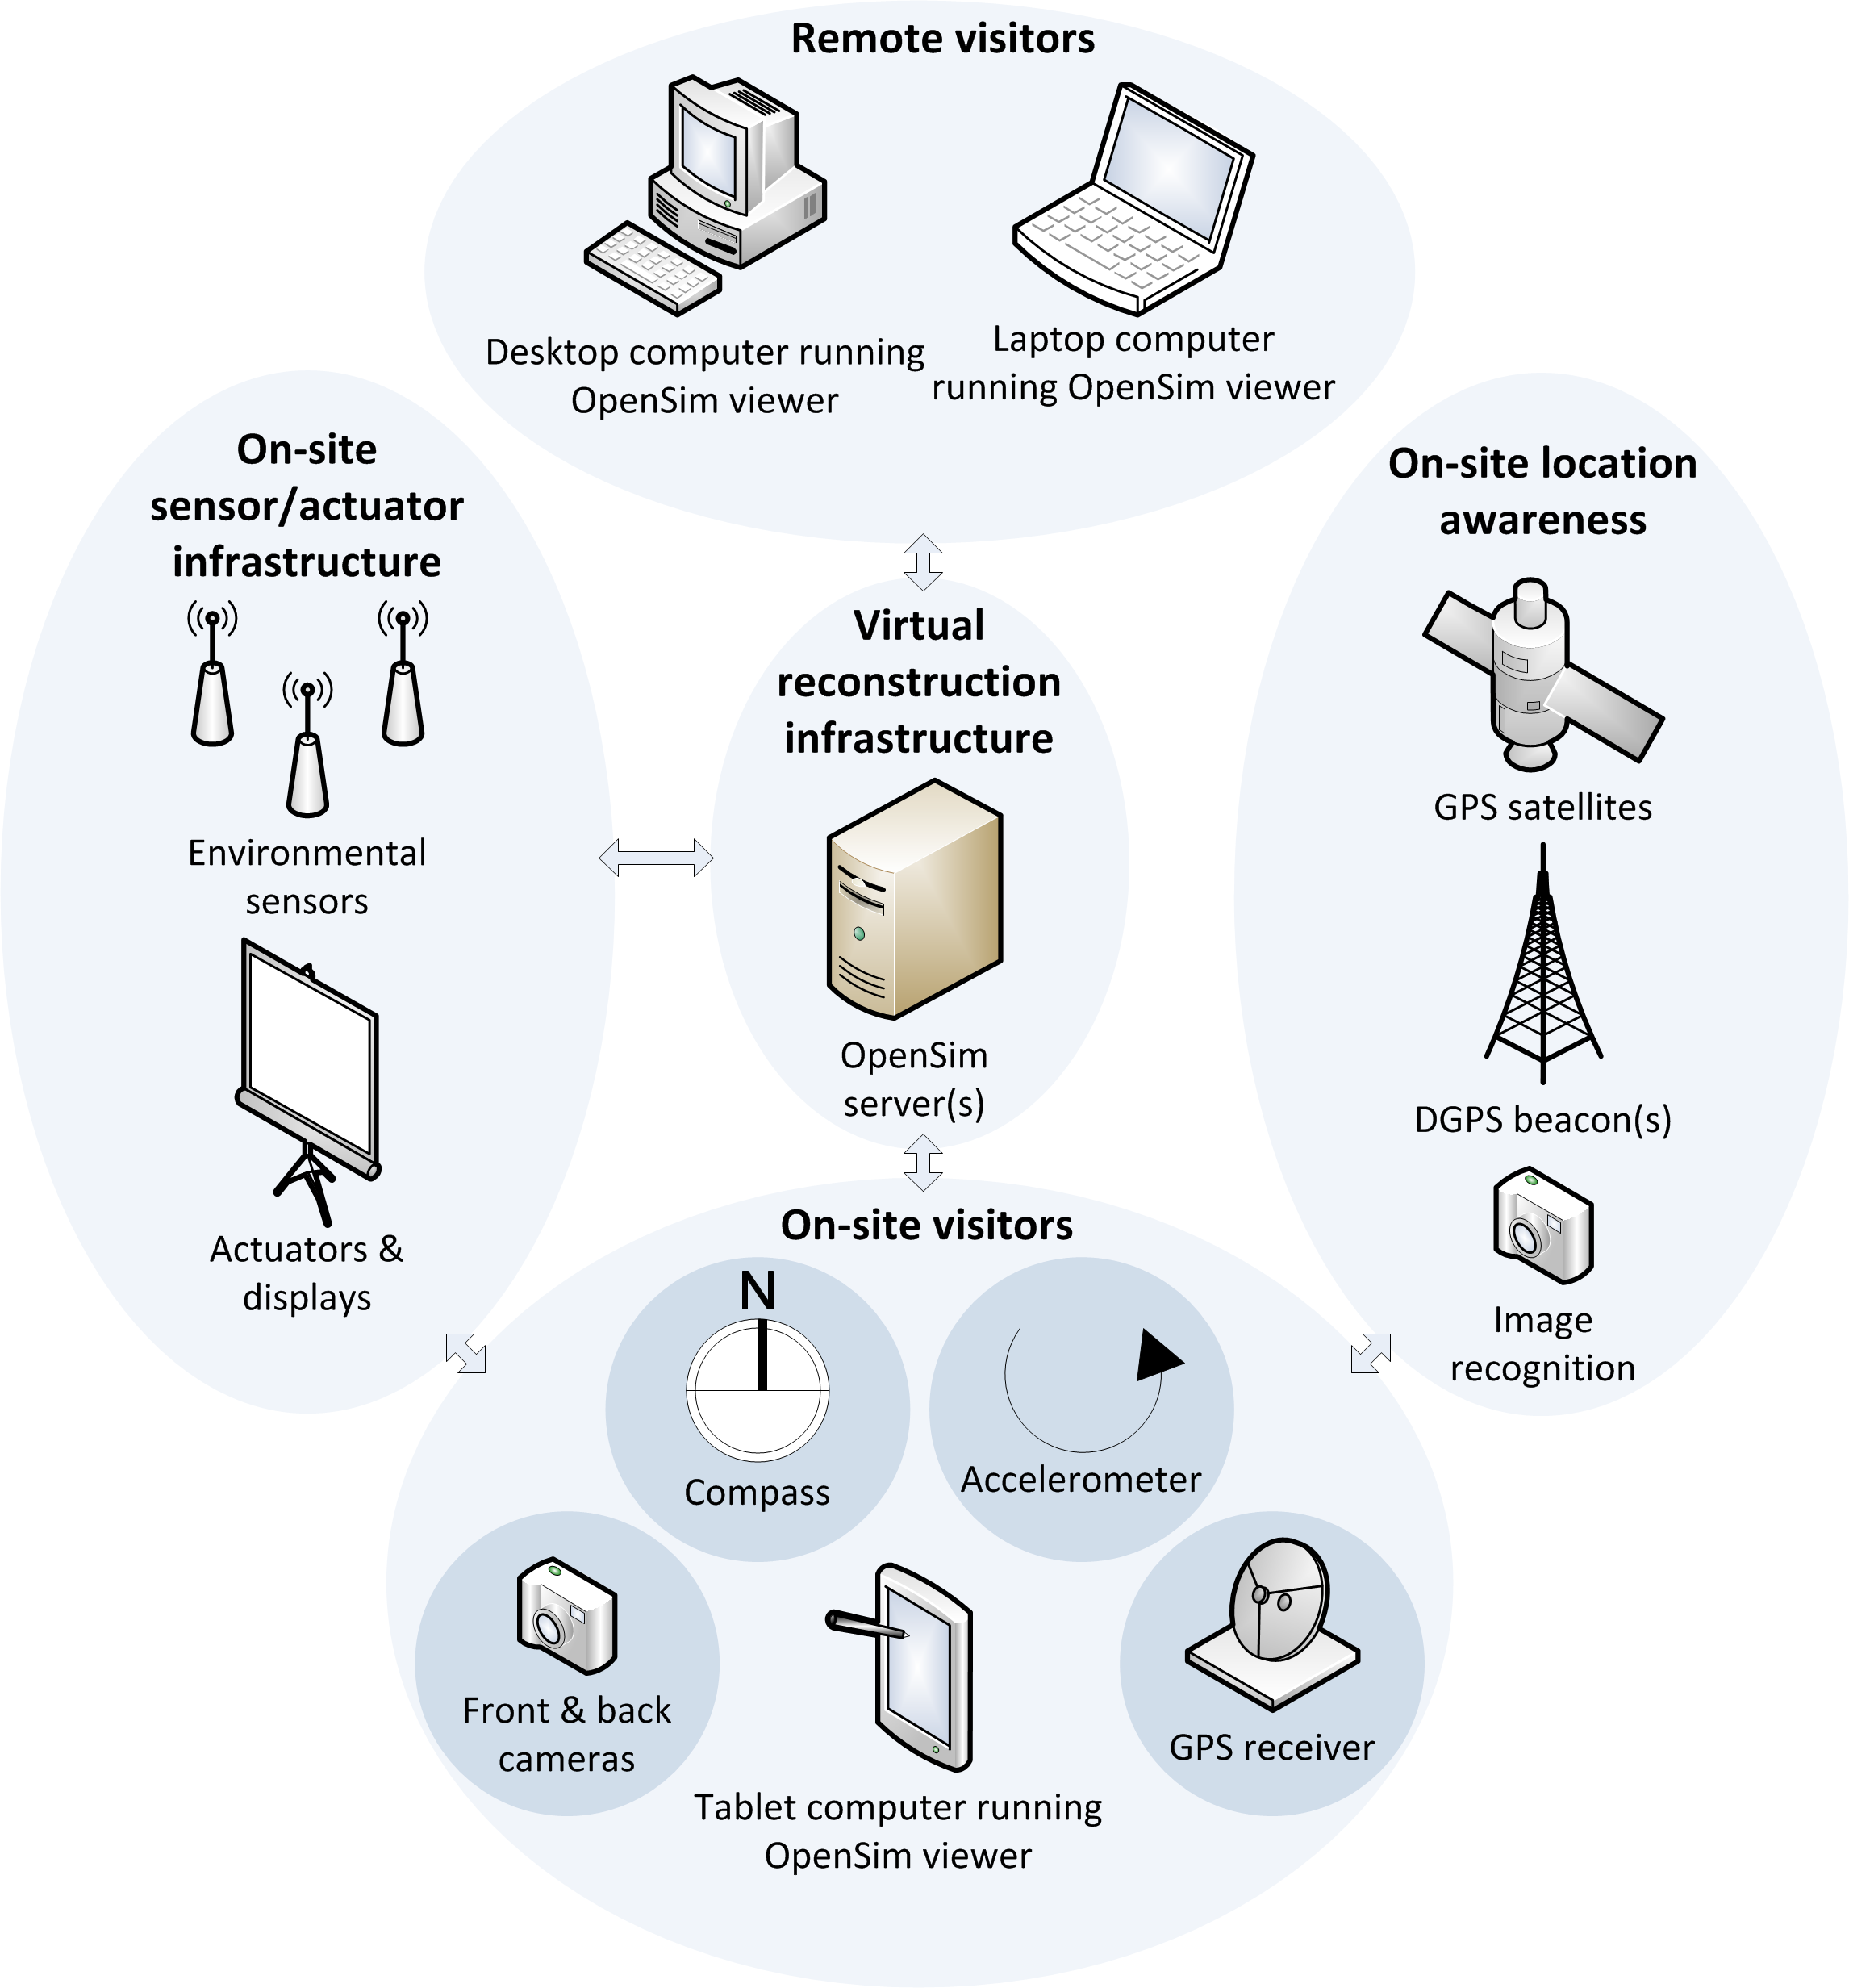
\includegraphics[width=0.48\textwidth]{visio_diagram_2_tech.png}
\caption{The main functional components and technologies of VTW from a high level of abstraction.}
\label{vtwarchitecturediagram}
\end{figure}

Visitors are categorised as either on-site, that is people who are physically present at the site and simultaneously exploring both it and the virtual world, or remote, that is people who are exploring only the virtual world from a computer physically remote to the site.

\subsection{Implementation of VTW}
\label{subsec:architecturaldetailsofvtw}
This section describes in detail some of the constituent technologies that comprise VTW, including available platforms and their suitability with regards to the specific requirements of the project.

\subsubsection{Virtual Reconstruction Infrastructure}
VTW uses OpenSim to provide the 3D multi-user virtual environment. In addition to the rationale presented in section \ref{sec:crossreality}, the existence of our OpenSim recreation of St Andrews cathedral, coupled with our physical proximity to the real cathedral, presents an ideal environment for early development and testing, without having to devote time to content generation.

\subsubsection{Tablet Computers}
Tablet computers are used to display the virtual world reconstruction and other associated digital content to visitors using virtual world `viewer' software. Currently this software is only available for x86/x86\_64 platforms which limits which tablet computers can be used.

Although popular tablet computers running Apple's iOS and Google's Android operating systems are now available with sufficiently powerful processors and graphics cards to produce the 3D graphics that a viewer requires, these are ARM platforms which cannot run viewer software. VTW is being developed under the assumption that with the continued adoption of virtual worlds and the ever growing popularity of tablet computers, increasing in computational power and decreasing in cost with every new release, viewers compatible with ARM platforms will become available before the project's completion. Until such a time we are using a MSI Windpad 110W 10'' tablet computer that sports an AMD Fusion Z-Series APU (dual core x86\_64 processor with Radeon HD6250 graphics).

Additional hardware considerations when determining a tablet computer's suitability for VTW is the presence of and/or compatibility with GPS, digital compass, accelerometer and camera hardware. Many tablet computers have some or all of these features built in and they can also be connected via wired or wireless connections.

\subsubsection{On-Site Sensor/Actuator Infrastructure}
Numerous hardware and software platforms exist that are suitable for adding sensing and actuating capabilities to a cultural heritage site~\cite{Bose2009}.

Hardware platforms include those designed specifically for the task of distributed sensing, such as wireless sensor network (WSN) solutions including Berkeley motes~\cite{Bose2009}, but there are also many general-purpose prototyping and embedded platforms that have proven popular for the creation of bespoke transducer devices, including Phidgets~\cite{Faludi2010, PhidgetsInc.} and Arduino~\cite{Faludi2010, Arduino}. The newly released Raspberry Pi~\cite{Foundation} promises to continue this trend.

Software platforms include operating systems tailored specifically for operation on WSN motes such as TinyOS ~\cite{TinyOSAlliance} and more general purpose operating systems such as Contiki~\cite{Dunkels} which is designed for running on devices with limited memory footprints and computational capabilities.

In addition to a dedicated sensing infrastructure, VTW may also make use of sensors built into the tablet computers carried by visitors and even the sensors built into other devices that these visitors may be carrying, such as smartphones.

Actuators will primarily serve as interfaces to controllable luminaires, fans, animatronics, etc. but also to more `traditional' output devices such as monitors, projectors and loudspeakers.

The obvious conclusion from even such a brief look into the range of suitable transducer platforms is that for VTW to be successful it must be able to integrate with as many of these platforms as possible, through standard interfaces that are not specific to any particular platform. The issue of standards in VTW is discussed further in section \ref{subsec:standards}.

\subsubsection{Networking}
VTW requires communication between a server and both on-site and off-site clients.

It is unrealistic to expect on-site clients to communicate directly with an off-site server via 3G cellular networks, as the speeds attainable are not high enough for a satisfactory experience and the costs incurred by large data transfers over these networks are prohibitive. 4G/WiMAX adoption has not yet reached a point where it is a viable alternative (at least in the UK). Thus it is envisaged that the site must have connectivity to the Internet via DSL, fibre, etc., and that the site will have LAN connectivity for clients to communicate with each other and with the server.

In this scenario the server can be situated either on-site or off-site (such as in a data centre). In the former case, on-site clients will communicate directly with the server via LAN, whilst in the latter case they will communicate via LAN to an on-site gateway which then mediates communication to the server via the Internet connection. Off-site clients will communicate with the server via the Internet in both cases.

LAN connectivity will include 802.11 wireless for communication to/from tablet computers and may also include other LAN technologies for communication with transducer infrastructure; many WSN/transducer platforms make use of low-power radio technologies such as ZigBee, instead of 802.11, whilst static actuators (for example those controlling mains-powered equipment such as luminaires) could make use of wired ethernet instead of 802.11.

The requirement for Internet connectivity restricts which sites are suitable for full VTW deployment as many are situated in remote areas with no connection to PTSN or fibre networks and the lag inherent with satellite communication renders it non-viable as an alternative. However there are enough sites that already have Internet connectivity to maintain VTW's viability. In addition, a `reduced' version of VTW that features an on-site server and does not support off-site visiting could be deployed at sites that lack Internet connectivity. Looking to the future, greater adoption of 4G/WiMAX will alleviate this issue.

\subsection{Standards in VTW}
\label{subsec:standards}
As mentioned in section \ref{sec:introduction} there are currently no widely adopted standards that are aimed specifically at the development of cross reality systems. This situation presents a serious challenge to the greater realization of the paradigm through projects such as VTW.

However the advent of the cross reality paradigm did not spawn the demand for such standards, that facilitate synchronous bidirectional flow of sensory and control information between transducer infrastructure and display technologies (be that display a virtual world or a traditional two-dimensional graph). This style of interaction has existed for a long time, as transducer networks were employed by numerous fields long before the adoption of virtual worlds as a research tool. As such there exist a plenitude of projects and standards that already facilitate bidirectional communication of sensory and control information to and from networks of transducers. These technologies include, but are not limited to;

\begin{itemize}

	\item{\bf{IEEE 1451}} $-$ A family of Smart Transducer Interface Standards defining a set of open, common, network-independent communication interfaces for connecting transducers to microprocessors, instrumentation systems and control/field networks~\cite{lee:standard}. The main goal of IEEE 1451 is to allow network access to standardised transducer data through a common set of interfaces, whether the transducers are connected to systems or networks via wired or wireless means~\cite{Song2008}.

	\item{\bf{Open Geospatial Consortium (OGC) Sensor Web Enablement (SWE)}} $-$ Aims to enable all Web and/or Internet accessible sensors (including imaging devices such as surveillance cameras) to be accessible and controllable via the Web, through open Web standards, creating in effect a `sensor Web' that can be accessed in a similar manner as to how HTML and HTTP allow access to the WWW. SWE harmonizes with other relevant sensor and alerting standards including IEEE 1451, the OASIS Common Alerting Protocol and Asynchronous Service Access Protocol, and Web Services Notification~\cite{Botts2008a}.

	\item{\bf{Ubiquitous Sensor Network (USN)}} $-$ A conceptual network built over existing physical network infrastructure, both traditional wired and wireless networks as well as WSNs, that makes use of sensed data and derived knowledge services available to anyone, anywhere and at any time. The importance of supporting USN applications and services in the Next Generation Network (NGN) environment has been recognised and addressed by the ITU with the publication of Rec.ITU-T Y.2221~\cite{ITU2010}. USN middleware, to address the inherent heterogeneity of sensor devices and the the data that they produce, was recognised as a key technology to propel the realization of the cross reality paradigm~\cite{kim:practical}.

	\item{\bf{Microsoft SenseWeb}} $-$ A system that allows peer production of sensing applications, producing new kinds of media and applications over existing data networks, by allowing users to grant access to their sensors to other remote users. Contributors deploy their own sensors, uploading their observations to the SenseWeb system, where they can then be accessed by other SenseWeb users through an application-specific GUI, allowing applications to initiate and access sensor data streams from shared sensors across the entire Internet~\cite{Kansal2007}.

	\item{\bf{EPFL Global Sensor Network (GSN)}} $-$ Middleware developed to support the rapid and simple deployment of a wide range of sensor network topologies, facilitate the flexible integration and discovery of sensor networks and sensor data, enable fast deployment and addition of new platforms, provide distributed querying, filtering and combination of sensor data and support dynamic adaptation of the system configuration during operation~\cite{Aberer2006}. GSN's key abstraction is the `virtual sensor', which abstracts from implementation details of access to sensor data and corresponds either to a data stream received directly from a sensor or to a data stream derived from other virtual sensors.

\end{itemize}

Existing implementations of the cross reality paradigm have tended to either adapt these existing standards and frameworks to fit their requirements, or more often have developed their own bespoke and proprietary intercommunications solutions. This latter approach results in systems that frequently are only compatible with a particular transducer or virtual environment platform and cannot be easily extended or used as a basis for future systems.

\subsection{MPEG-V}
The most promising work toward alleviating the standards situation is MPEG-V, a unified effort begun in 2007 to develop standards for communication between different virtual worlds and between virtual worlds and the real world. This work culminated in the publication of ISO/IEC 23005 `Information technology $-$ Media context and control' in January 2011.

\begin{quotation}
	\textit{``The `Information exchange with Virtual Worlds' project intends to provide a standardized global framework and associated interfaces, intermediate formats definitions and the like, to enable the interoperability between virtual worlds... ...and between virtual worlds and the real world''}~\cite{Gelissen2008}
\end{quotation}

In the first instance VTW will make use of MPEG-V wherever possible, ensuring maximum compatibility with different transducer and virtual environment platforms, ensuring maximum extensibility by other interested parties and serving as an example of what can be achieved with the new framework. This process will likely involve the creation of interfaces that allow standards such as those listed above to communicate with VTW's implementation of MPEG-V features, to maximise support for legacy systems.

\section{Conclusions}
In this paper we have provided an overview of the cross reality paradigm; we have defined it, recounted its history and described its relation to other alternate realities that computer scientists have previously explored. In brief, cross reality is the situation that arises when augmented reality and augmented virtuality take place in unison; sensor readings from a real world location trigger effects in a virtual environment whilst actions within this virtual environment simultaneously manifest into the real world via displays and actuators.

We have identified several fields that we believe can benefit from the paradigm, as well as surveying several commercial and research examples where it has already been applied. We argue that the domain of cultural heritage is particularly well suited to benefit and propose such a project, applying the paradigm to the simultaneous exploration of real cultural heritage sites and their virtually recreated counterparts using a tablet computer in combination with transducer infrastructure and the OpenSim virtual world platform.

%\end{document}  % This is where a 'short' article might terminate

%
% The following two commands are all you need in the
% initial runs of your .tex file to
% produce the bibliography for the citations in your paper.
\bibliographystyle{abbrv}
\bibliography{bib}  % bib.bib is the name of the Bibliography in this case
% You must have a proper ".bib" file
%  and remember to run:
% latex bibtex latex latex
% to resolve all references
%
% ACM needs 'a single self-contained file'!

%\balancecolumns % GM June 2007
% That's all folks!
\end{document}